\chapter{TikZ}

\targets{
  \item Erstes Ziel
  \item Zweites Ziel
  \item Drittes Ziel
  \item Viertes Ziel
}

\website

\section{Einführung}

\begin{Frame}{Was ist \TikZ?}
  \begin{itemize}
    \item \TikZ\ ist kein Zeichenprogramm.
    \item \dots
  \end{itemize}
\end{Frame}

\begin{Frame}{Ein erstes Beispiel}
  \begin{center}
    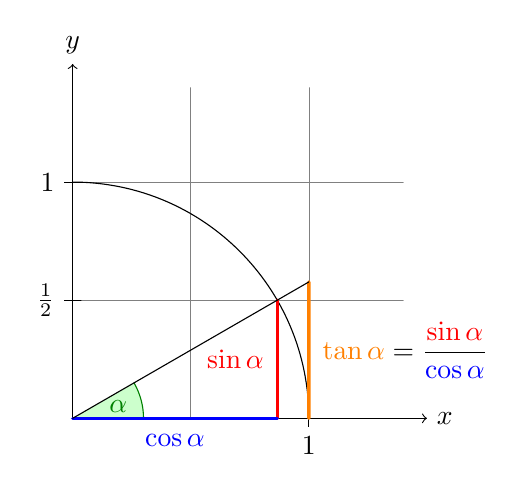
\begin{tikzpicture}[scale=3,line cap=round]
      \draw[help lines,step=0.5cm] (0,0) grid (1.4,1.4);
      \draw (1,0) arc (0:90:1cm);

      \draw[->] (0,0) -- (1.5,0) node[right] {$x$} coordinate(x axis);
      \draw[->] (0,0) -- (0,1.5) node[above] {$y$} coordinate(y axis);
      \draw[xshift=1cm] (0pt,1pt) -- (0pt,-1pt) node[below,fill=white] {$1$};
      \draw[yshift=0.5cm] (1pt,0pt) -- (-1pt,0pt) node[left,fill=white] {$\frac{1}{2}$};
      \draw[yshift=1cm] (1pt,0pt) -- (-1pt,0pt) node[left,fill=white] {$1$};
      
      \filldraw[fill=green!20,draw=green!50!black] (0,0) -- (3mm,0pt) arc(0:30:3mm);
      \draw (15:2mm) node[green!50!black] {$\alpha$};
      \draw[very thick,red]
        (30:1cm) -- node[left=1pt,fill=white] {$\sin \alpha$} (30:1cm |- x axis);
      \draw[very thick,blue]
        (30:1cm |- x axis) -- node[below=2pt,fill=white] {$\cos \alpha$} (0,0);
      \path [name path=upward line] (1,0) -- (1,1);
      \path [name path=sloped line] (0,0) -- (30:1.5cm);
      \draw [name intersections={of=upward line and sloped line, by=t}]
        [very thick,orange] (1,0) -- node [right=1pt,fill=white]
        {$\displaystyle \tan \alpha \color{black}=
          \frac{{\color{red}\sin \alpha}}{\color{blue}\cos \alpha}$} (t);
      \draw (0,0) -- (t);
    \end{tikzpicture}
  \end{center}
\end{Frame}

\subsection{Verwendung}

\begin{Frame}[fragile]{\TikZ\ verwenden}
  \begin{lstlisting}[gobble=4]
    \documentclass{scrartcl}
    \usepackage{tikz}
    \usetikzlibrary{intersections}
    \begin{document}
      Wir arbeiten an
      \begin{tikzpicture}
        \draw (0,0) -- (1.5,0);
        \draw (0,0) -- (0,1.5);
      \end{tikzpicture}.
    \end{document}
  \end{lstlisting}

  \xxx

  Wir arbeiten an
  \begin{tikzpicture}
    \draw (0,0) -- (1.5,0);
    \draw (0,0) -- (0,1.5);
  \end{tikzpicture}.
\end{Frame}

\subsection{Pfade}

\begin{Frame}[fragile]{Pfade}
  \begin{itemize}
    \item Ein Pfad ist eine Folge von Koordinaten.
      \begin{itemize}
        \item Links unten ist \lstinline-(0,0)-,
        \item die erste Koordinate geht nach rechts und
        \item die zweite Koordinate geht nach links.
      \end{itemize}
    \item Eine Linie wird mit \lstinline|--| gezeichnet.
    \item Relative Koordinaten beginnen mit \lstinline-++-.
  \end{itemize}

  \xxx

  \begin{lstlisting}[gobble=4]
    \draw[thick]
      (0,0) -- ++(1,0) ++(0,1) -- ++(-1,0)
      (2,0) rectangle (3,1);
  \end{lstlisting}

  \begin{center}
    \begin{beamercolorbox}{examplecolor!10}
      
\begin{tikzpicture}
        \draw[thick]
          (0,0) -- ++(1,0) ++(0,1) -- ++(-1,0)
          (2,0) rectangle (3,1);
      \end{tikzpicture}
    \end{beamercolorbox}
  \end{center}
\end{Frame}

% weitere Striche

\section{Graphen}

\subsection{Knoten}

\subsection{Automaten}

\section{Fortgeschrittene Verwendung}

\subsection{Funktionen plotten}

\subsection{Animationen mit Beamer}

\section*{Zusammenfassung}

\begin{frame}{Zusammenfassung}
  \begin{enumerate}
    \item Zusammenfassung.
  \end{enumerate}
\end{frame}